\bibliography{dissertation}
\appendix

\chapter{AI Usage}
\label{appx:ai_prompt}

I did not directly prompt any Large Language Models, or any other AI model, to assist with the writing of my dissertation or implementation. However, as listed in the Supporting Technologies list, I used GitHub Copilot to help with writing some tests for the parser and type checker. I used it via the VS Code extension, which uses the context of your file, to provide advanced AI autocompletion.

% =============================================================================

\chapter{Tokens for Lexical Analysis}
\label{appx:tokens}
Below is the code for how tokens outputted by lexical analysis are defined. 
\begin{lstlisting}
enum TokenType {
    EOF,
    Newline,

    Id,
    UppercaseId,

    If,
    Then,
    Else,

    Match,
    LBrace,
    RBrace,

    IntLit,
    FloatLit,
    StringLit,
    CharLit,
    BoolLit,

    DoubleColon,
    RArrow,
    Forall,
    KWType,
    KWData,

    LParen,
    RParen,

    Lambda,

    Dollar,
    Dot,
    Comma,
    Bar,

    Assignment,
}

struct Token {
    tt: TokenType,
    value: String,
}
\end{lstlisting}

\chapter{UI Screenshots}
\begin{figure}[h]
    \centering
    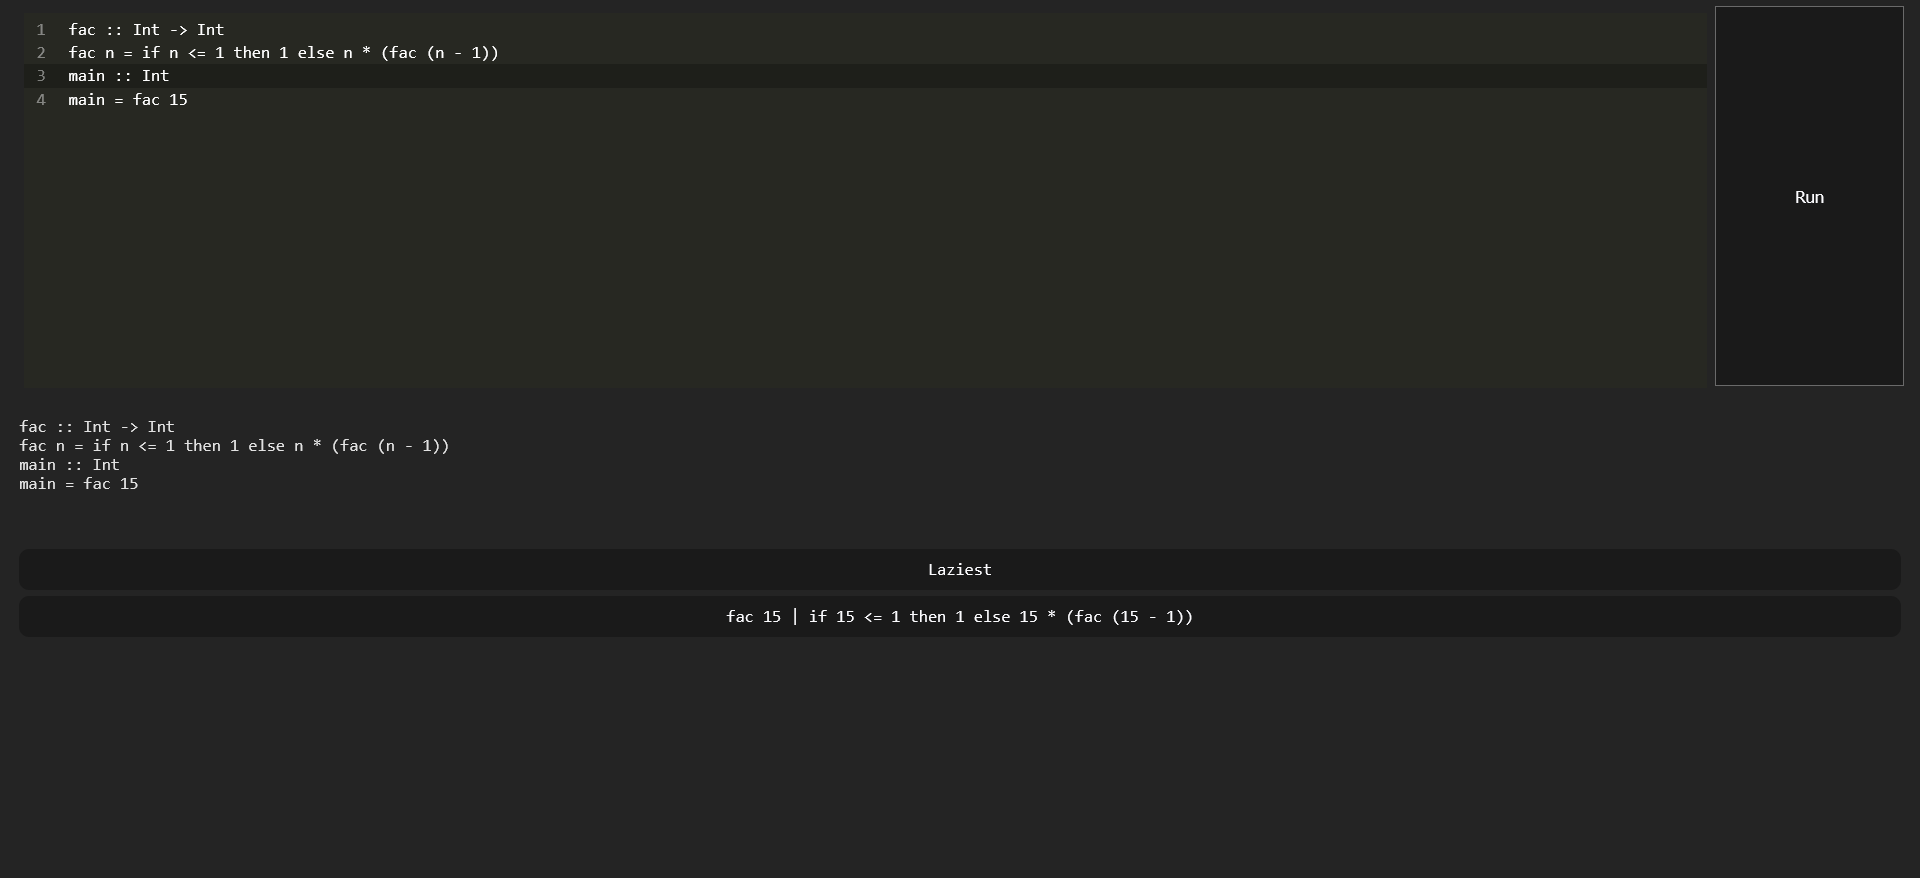
\includegraphics[width=1\linewidth]{images/cycle-1-end.png} 
    \captionsetup{justification=centering}
    \caption{The Web UI \ac{MVP}, as presented to my client at the end of cycle 1. Note that this does have type assignments, but these were just ignored by the parser and typechecker at this stage. }
    \label{fig:screenshot_cycle_1_end}
\end{figure}

\begin{figure}[h]
    \centering
    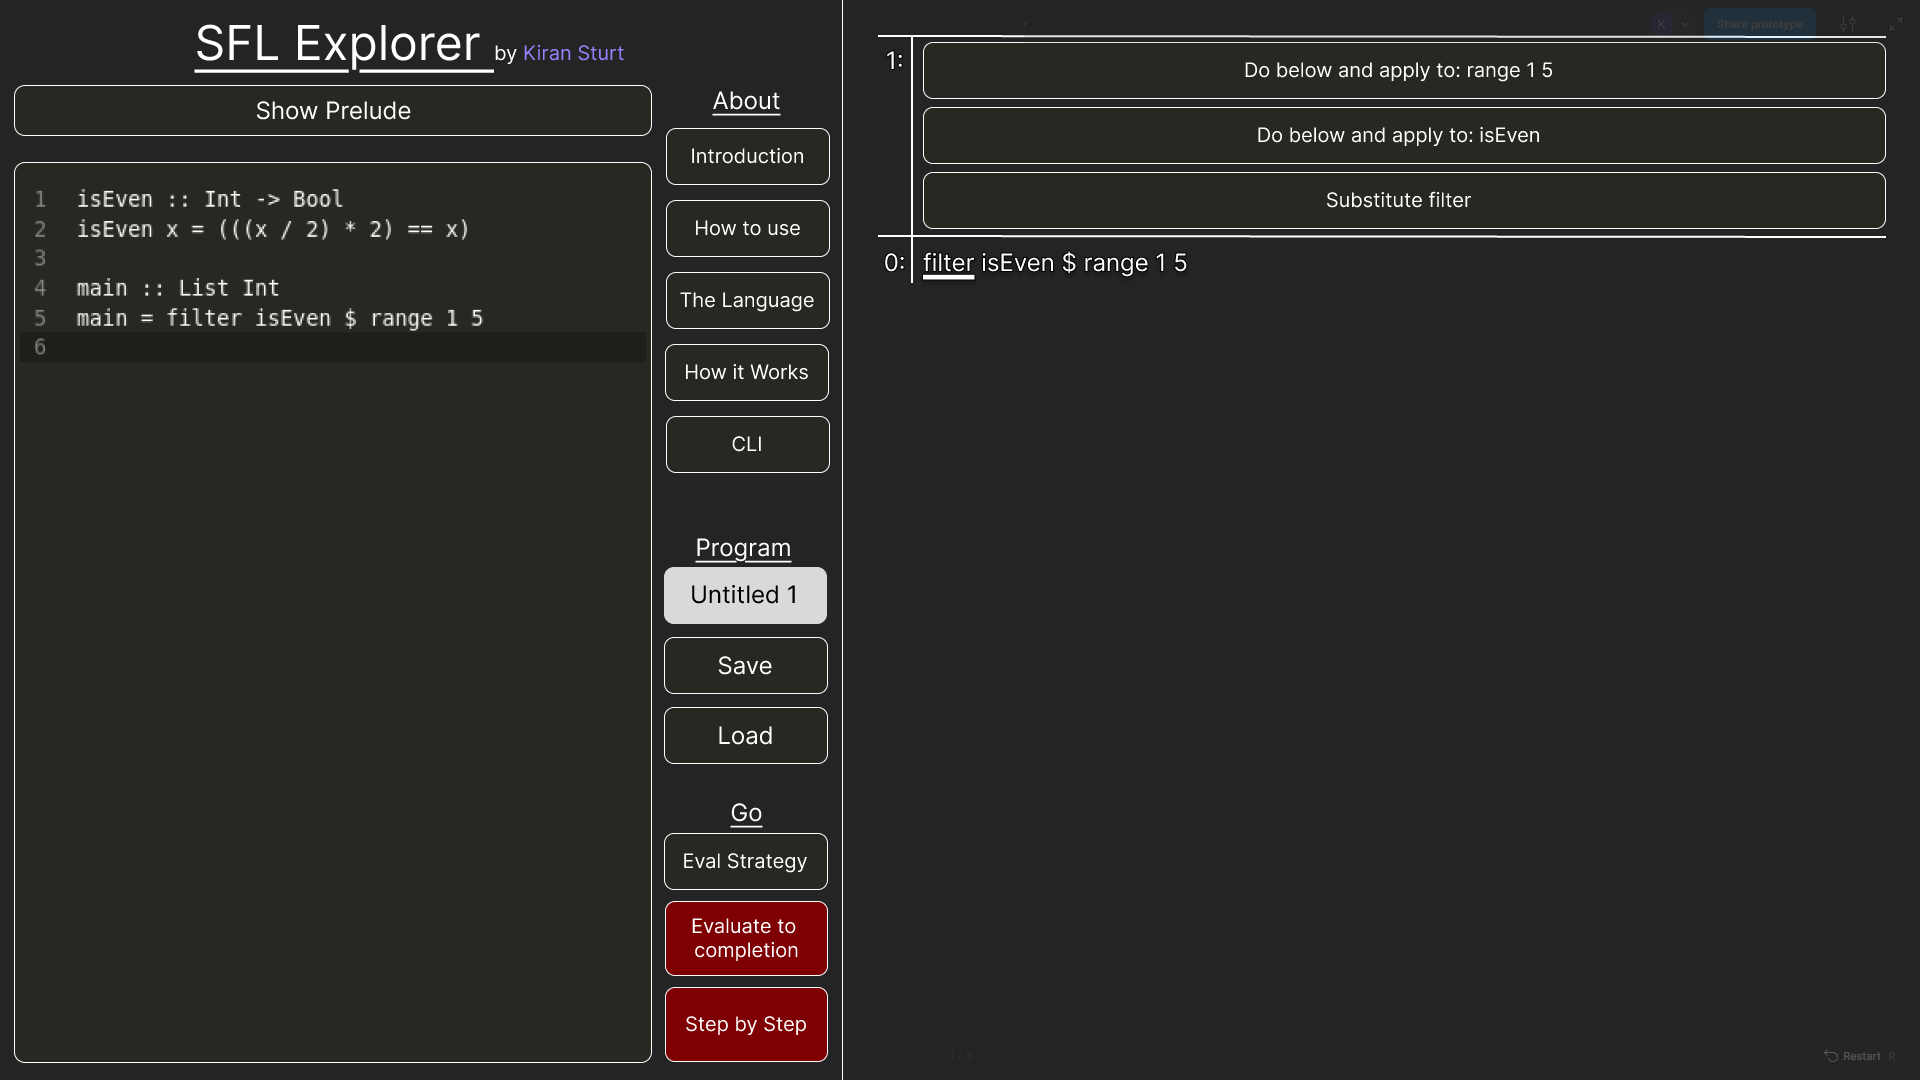
\includegraphics[width=1\linewidth]{images/figma_1.png} 
    \captionsetup{justification=centering}
    \caption{Screenshot 1 of the Figma design of the web UI}
    \label{fig:screenshot_figma1}
\end{figure}

\begin{figure}[h]
    \centering
    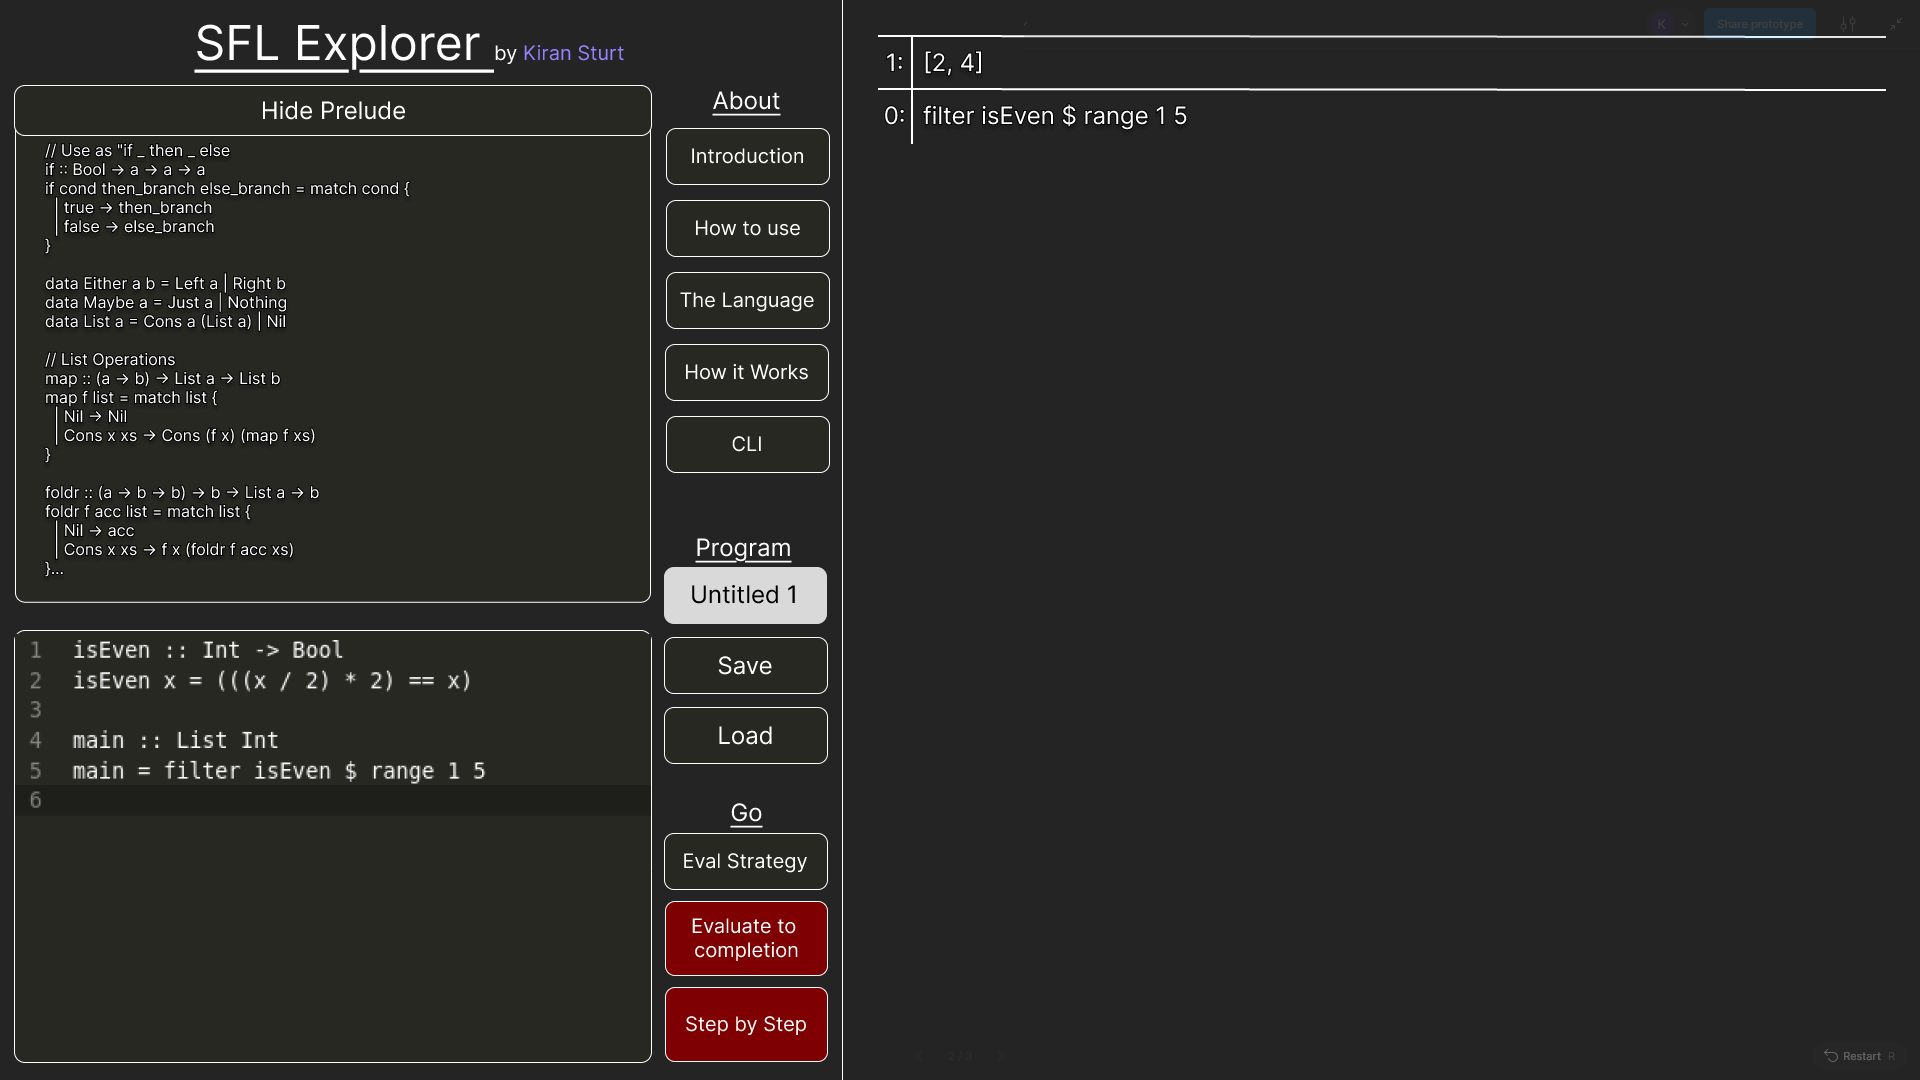
\includegraphics[width=1\linewidth]{images/figma_2.png}
    \captionsetup{justification=centering}
    \caption{Screenshot 2 of the Figma design of the web UI. This version shows the prelude extended}
    \label{fig:screenshot_figma2}
\end{figure}

\begin{figure}[h]
    \centering
    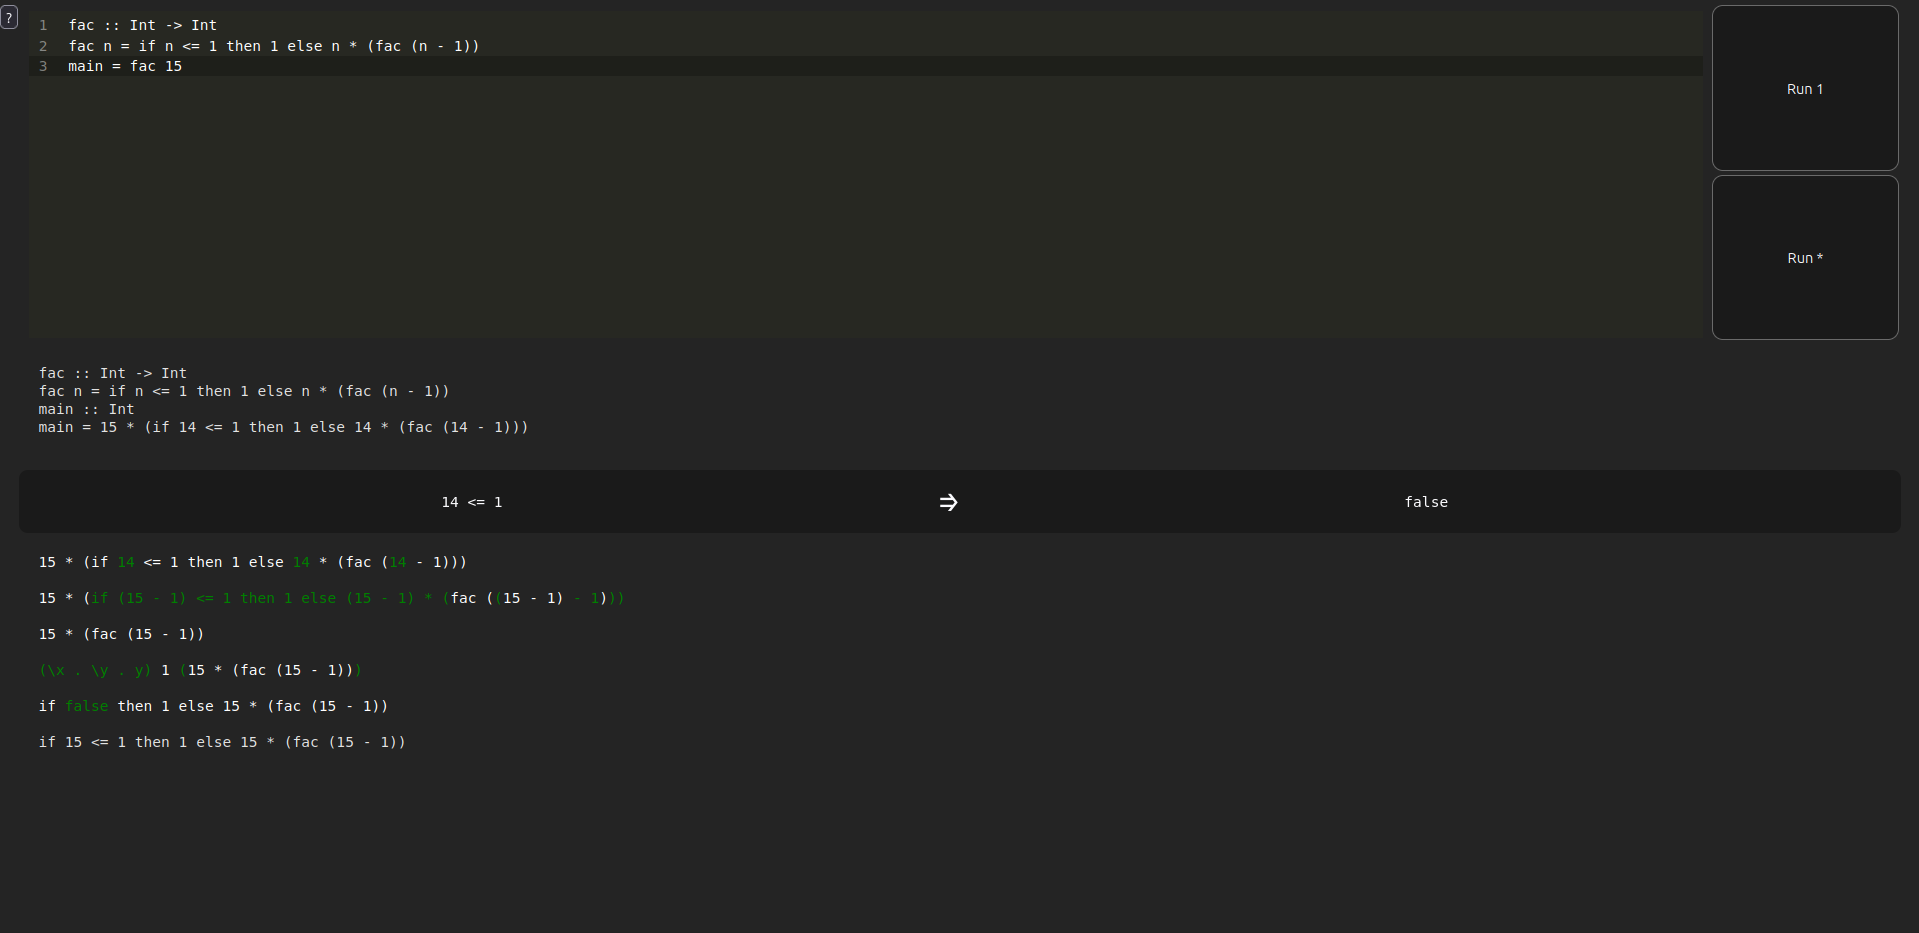
\includegraphics[width=1\linewidth]{images/product_at_testathon.png} 
    \captionsetup{justification=centering}
    \caption{The UI as tested in the testathon}
    \label{fig:screenshot_testathon}
\end{figure}

\begin{figure}[h]
    \centering
    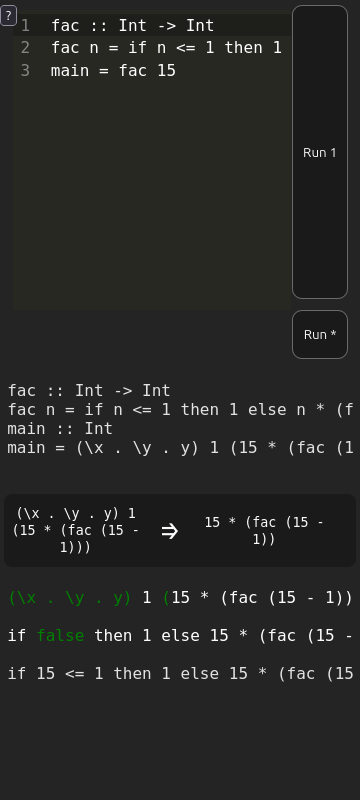
\includegraphics[width=0.3\linewidth]{images/testathon-mobile.png}
    \caption{The UI as tested in the testathon, as it would have appeared on a Samsung Galaxy S20}
    \label{fig:screenshot_testathon_mobile}
\end{figure}

\begin{figure}[h]
    \centering
    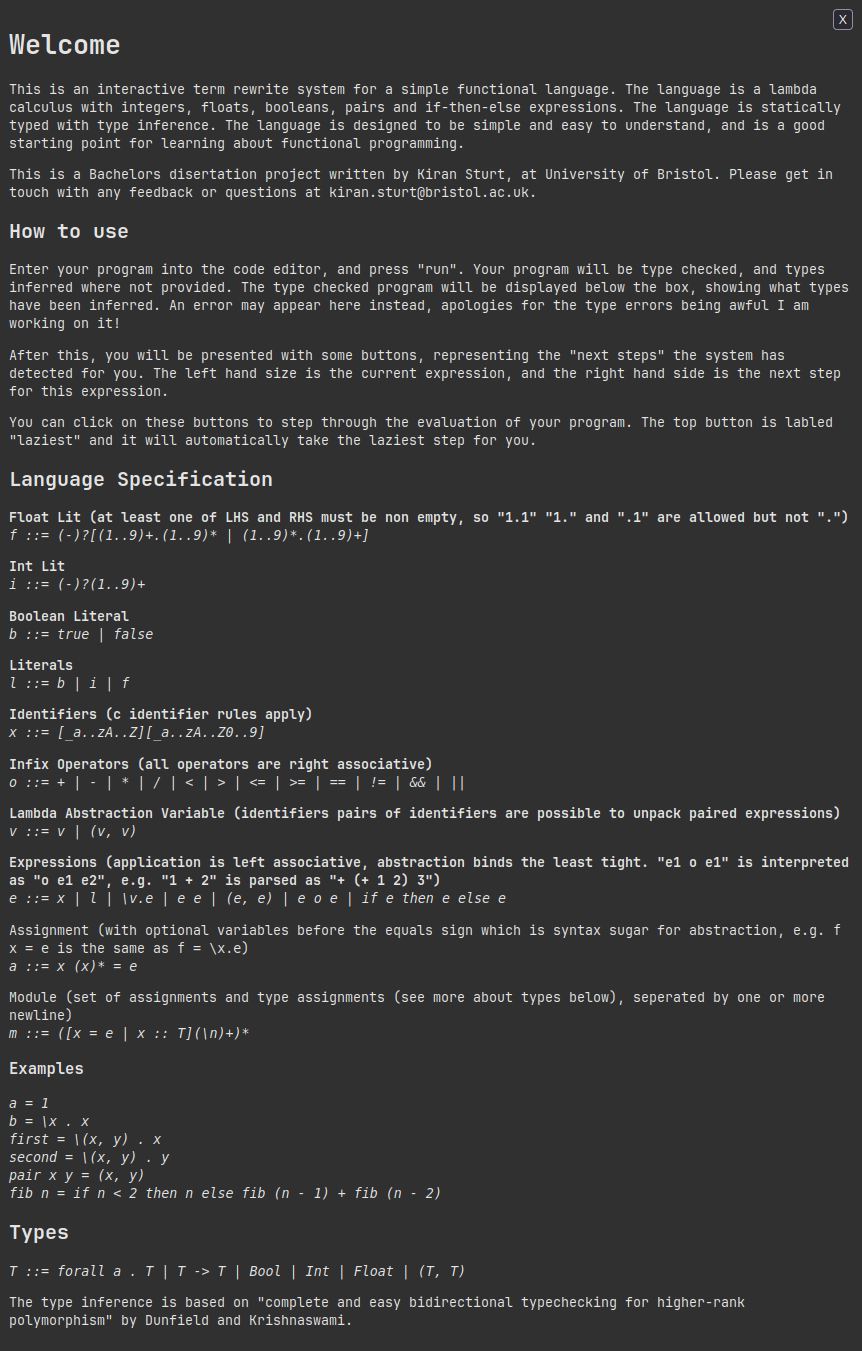
\includegraphics[width=0.9\linewidth]{images/testathon_help_menu_cropped.png} 
    \captionsetup{justification=centering}
    \caption{The "Help menu" in the testathon. This was spawned by pressing the "?" button in the top left of the UI, and dismissed by pressing the "X" button, or clicking outside of the box}
    \label{fig:screenshot_testathon_2}
\end{figure}

\begin{figure}[h]
    \centering
    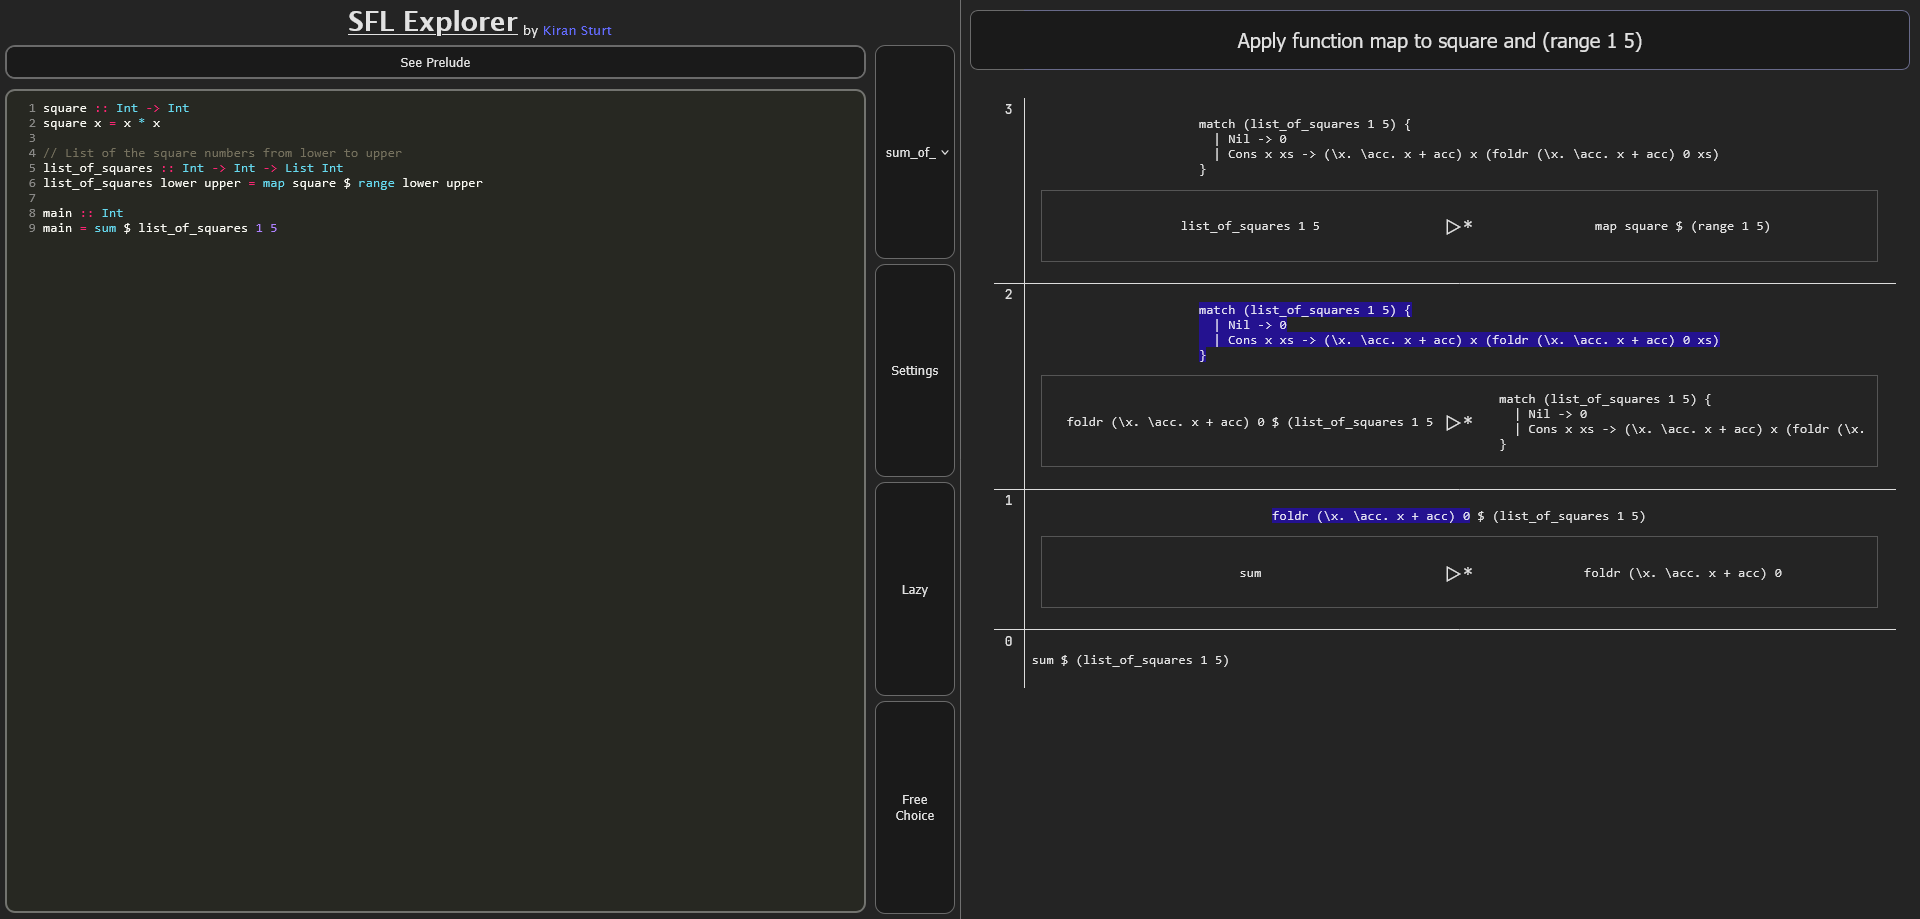
\includegraphics[width=\linewidth]{images/final_dark.png} 
    \captionsetup{justification=centering}
    \caption{The final product during lazy evaluation of the `sum of squares' sample program}
    \label{fig:screenshot_final_dark}
\end{figure}

\begin{figure}[h]
    \centering
    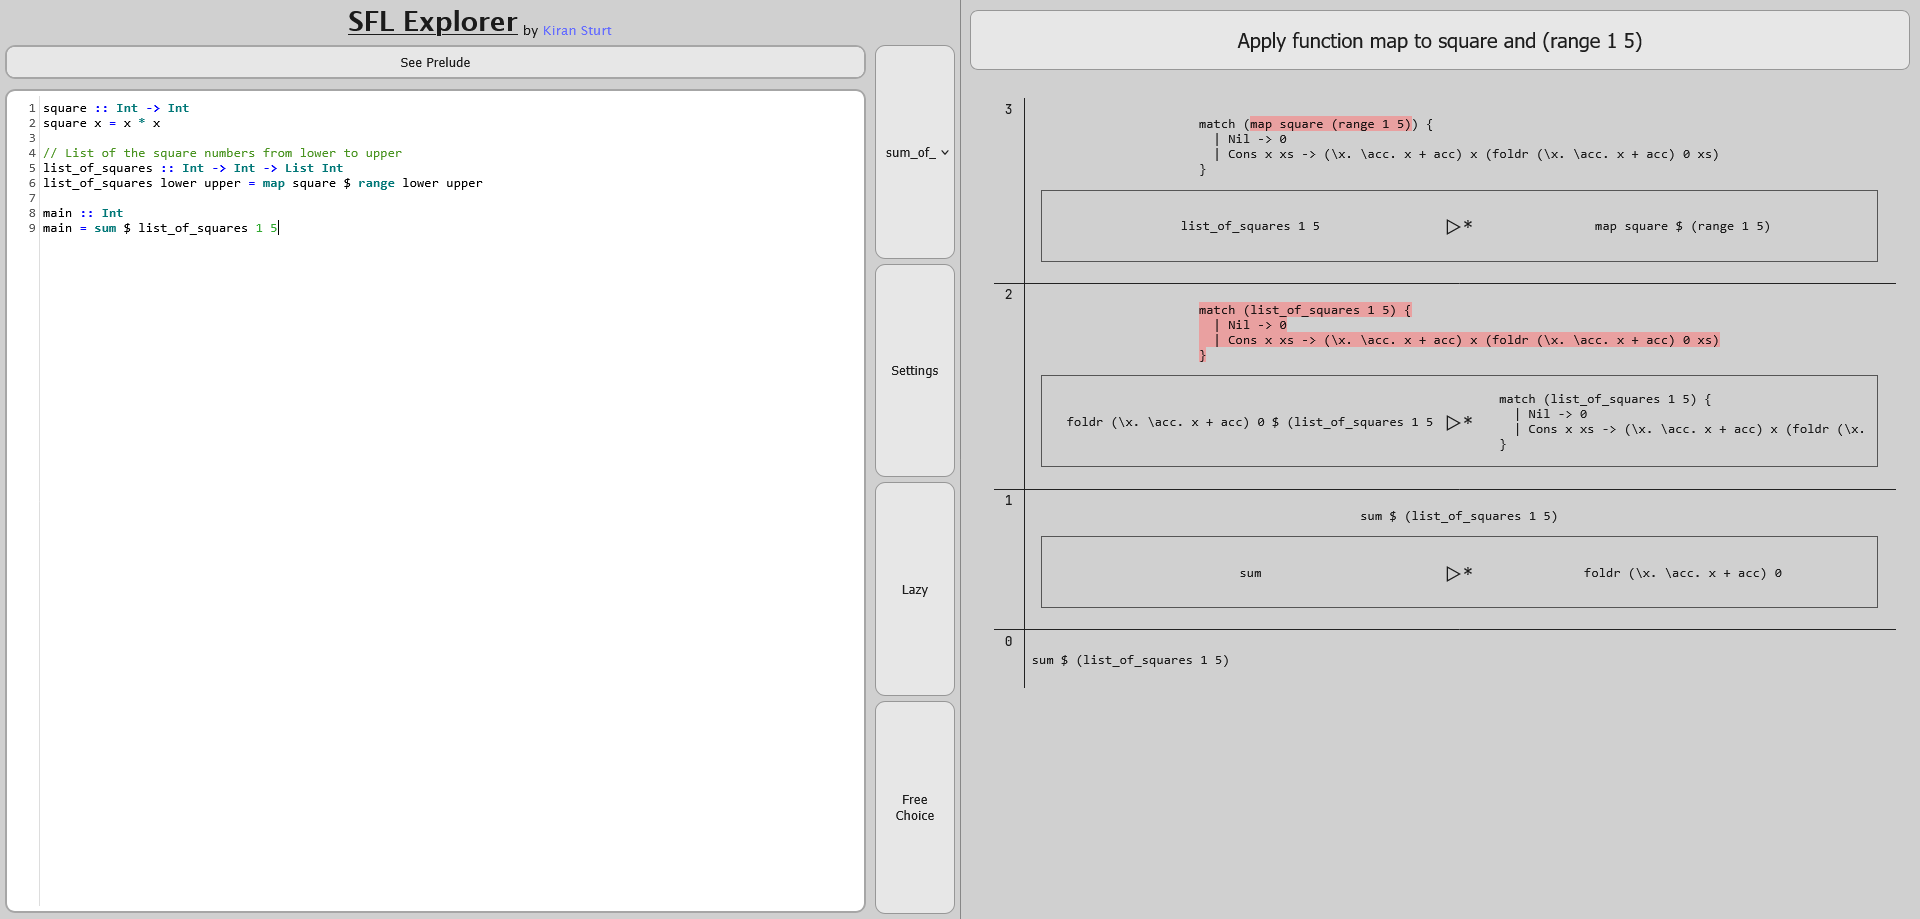
\includegraphics[width=\linewidth]{images/final_light.png} 
    \captionsetup{justification=centering}
    \caption{The final product during lazy evaluation of the `sum of squares' sample program in light mode}
    \label{fig:screenshot_final_light}
\end{figure}

\begin{figure}[h]
    \centering
    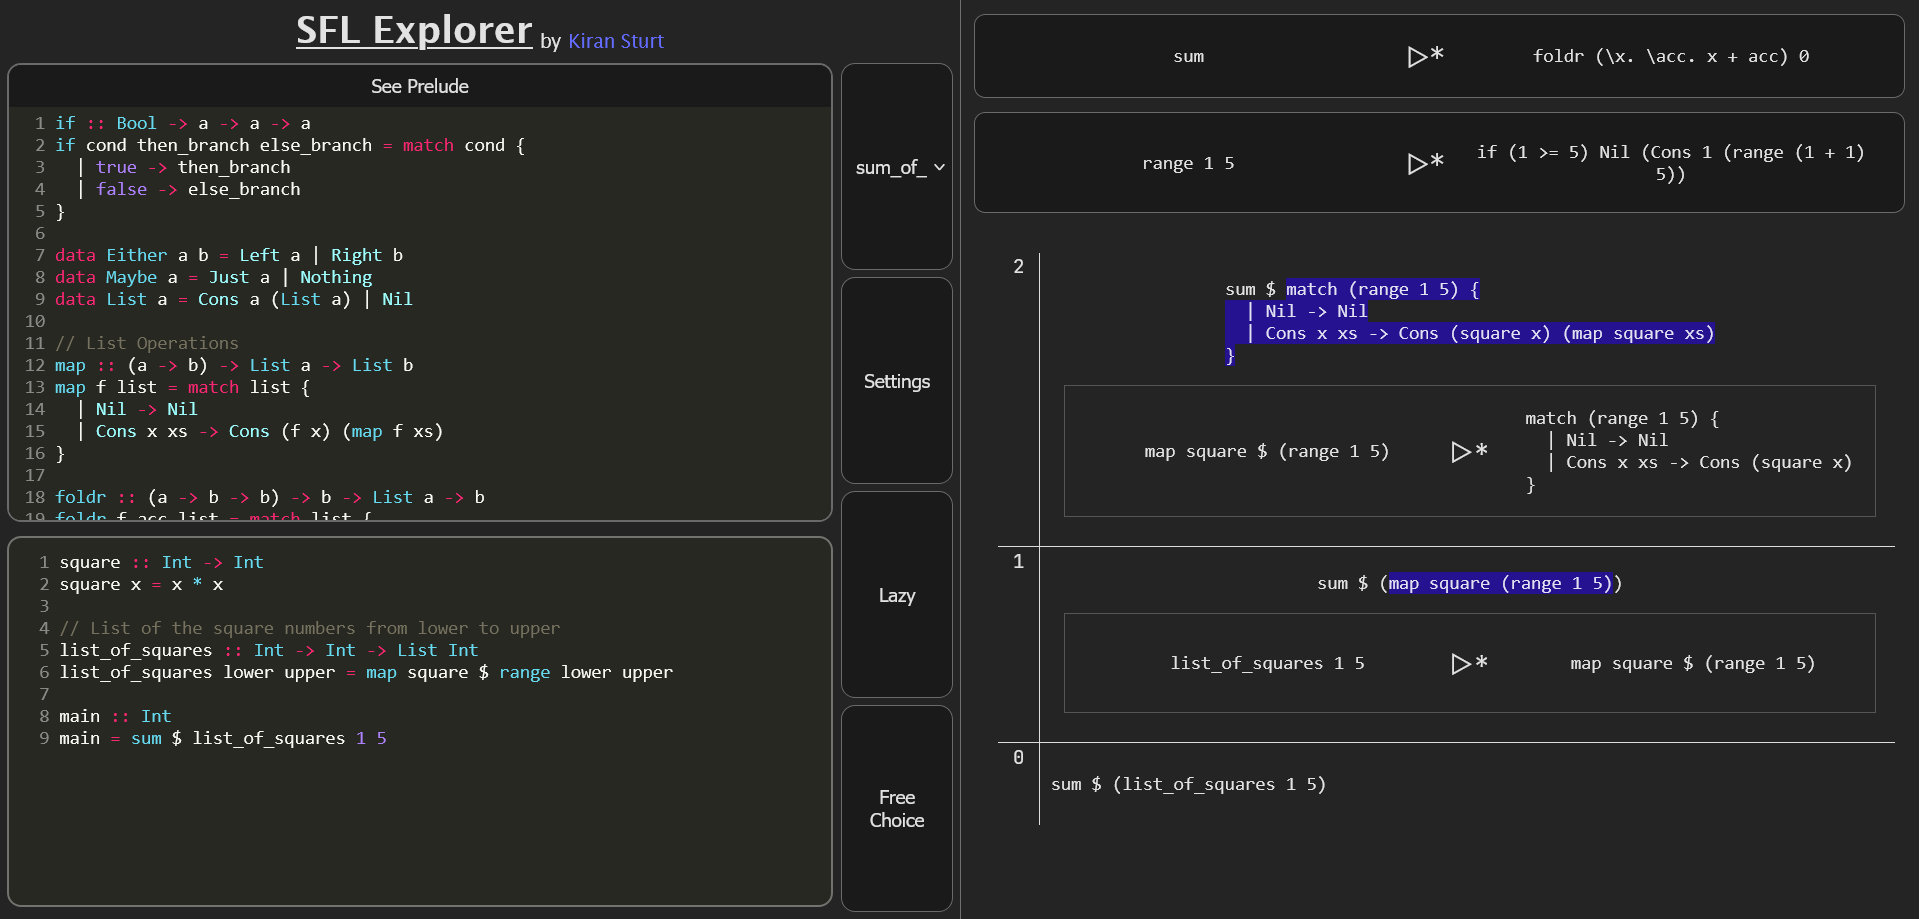
\includegraphics[width=\linewidth]{images/final_dark_prelude_free.png} 
    \captionsetup{justification=centering}
    \caption{The final product during free choice evaluation of the `sum of squares' sample program, with the prelude visible}
    \label{fig:screenshot_final_dark_prelude_free}
\end{figure}

\begin{figure}[h]
    \centering
    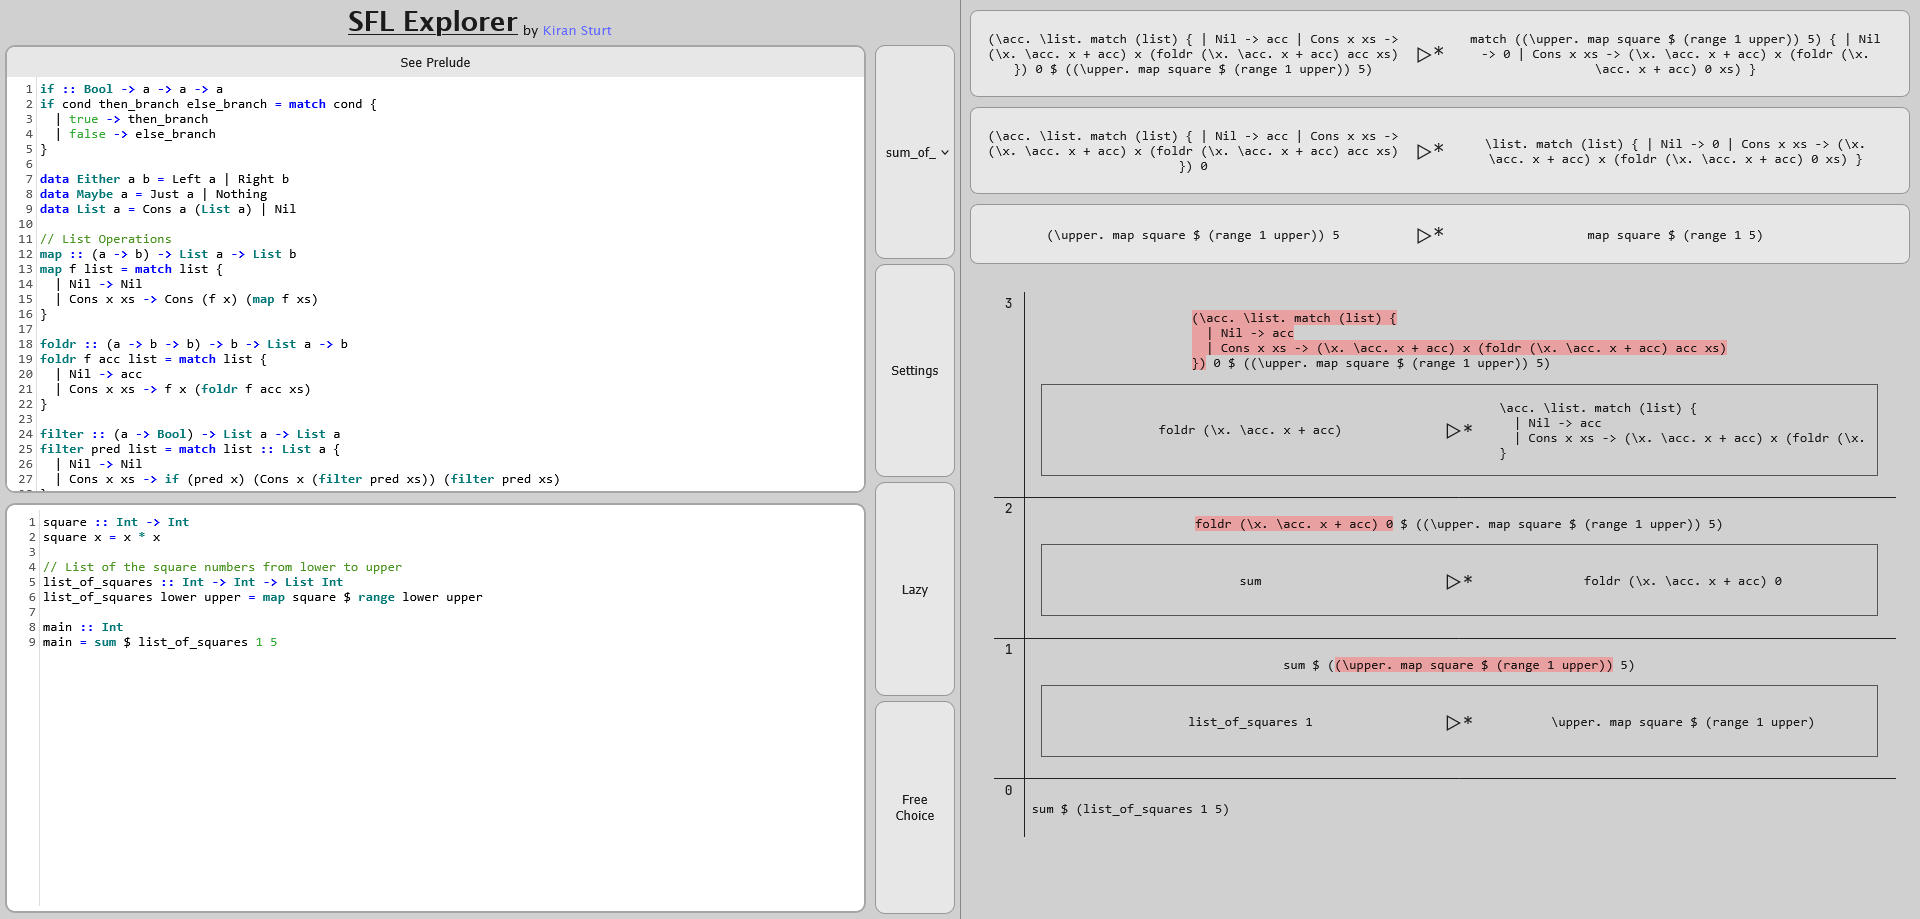
\includegraphics[width=\linewidth]{images/final_light_prelude_free.png} 
    \captionsetup{justification=centering}
    \caption{The final product during free choice evaluation of the `sum of squares' sample program, with the prelude visible in light mode}    
    \label{fig:screenshot_final_light_prelude_free}
\end{figure}

\chapter{Language Grammar}
\input{sections/lang_grammar}

\chapter{Some Example Derivations Using the Type Checking Algorithm}
\chapter{Some Example Derivations Using the Type Checking Algorithm}
\label{appx:example_derive}



% \section{Typechecking an Expression Involving Lists}
% We shall attempt to use the algorithm to check the type of $\text{Cons}\;1\;x$ against $Int \fto List\;Int$. This derivation will skip some trivial subtyping/instantiation, but it should serve as a demonstration of how more complex checking works. 

% \begin{mathpar}
% T_{Cons} = \alltype{\alpha}{\alpha \fto List\; \alpha \fto List\;\alpha}\\
% \Gamma_0 = T_{Cons}\and
% \Gamma_1 = \Gamma_0, \ahat, \bhat, x : \ahat \\

% \Infer{\Sub[1]}
%     {
%         [2]
%         \\
%         \subjudg{\Theta}{[\Theta]A}{[\Theta]B}{\Delta}
%     }
%     {\chkjudg{\Gamma}{\lam{x} Cons\;1\;x}{List\;Int}{\Delta}}

% \\

% {\Infer{{\!\ArrIntroSyn}[2]}
%     {
%     \chkjudg{\Gamma_1}{Cons\;1\;x}{\bhat}{\Delta, x : \ahat, \Theta}
%     }
%     {{\synjudg{\Gamma_0}{\lam{x} Cons\;1\;x}{\ahat \arr \bhat}{\Delta}}}

%     \Infer{\!\ArrElim[3]}
%         {
%         {
%             [4]{\synjudg{\Gamma_1}{Cons\,1}{C}{\Delta}}
%         }
%         \\
%         \appjudg{\Gamma_1}{x}{[\Gamma_1]A}{C}{\Delta}
%         }
%         {\synjudg{\Gamma}{Cons\,1\,x}{C}{\Delta}}
% }

% \\
% \Infer{\!\ArrElim[4]}
%     {
%     {
%     \Infer{\Var}
%         {(Cons : T_{Cons}) \in \Gamma_1}
%         {\synjudg{\Gamma_1}{Cons}{T_{Cons}}{\Gamma_1}}
%     }
%     \\
%     {
%      \Infer{\AllApp}
%         {\appjudg{\Gamma_1,\ahat}{1}{(\ahat \fto List\; \ahat \fto List\;\ahat)}{C}{\Delta}}
%         {\appjudg{\Gamma_1}{1}{\alltype{\alpha}{\alpha \fto List\; \alpha \fto List\;\alpha}}{C}{\Delta}}
%     }
%     }
%     {\synjudg{\Gamma_1}{Cons\,1}{C}{\Delta}}
% \end{mathpar}


\section{Typechecking an Expression Involving Lists}
We shall attempt to use the algorithm to check the type of $\text{Cons}\;1\;x$ against $List\;Int$. This derivation should serve as a demonstration of how more complex checking works. This derivation assumes $Cons$ and $Nil$ are defined over $Int$s only. The reason the context is never changed is as we do not have any abstractions or foralls, so no variables or type variables are introduced.

\begin{mathpar}
T_{Nil} = List\;Int\and
T_{Cons} = {Int \fto List\;Int \fto List\;Int}\\
\Gamma = T_{Cons}, T_{Nil}\and\Gamma = \Gamma_0 = \Gamma_1\\

\\

\Infer{\MyTCRule{\Unionsubrulename}[10]}
    {\Infer{\MyTCRule{\Intsubrulename}[11]}{ }
        {\subjudg{\Gamma_0}{\Inttype}{\Inttype}{\Gamma_1}}}
    {\subjudg{\Gamma_0}{List[Int]}{List[Int]}{\Gamma_{1}}}
\\

\Infer{\ArrApp[7]}
    {     \Infer{\Sub[8]}
          { 
          {
          \Infer{\Var[9]}
            {(Nil : T_{Nil}) \in \Gamma}
            {\synjudg{\Gamma}{Nil}{T_{Nil}}{\Gamma}}
          }
            \\
            [10]\subjudg{\Gamma}{List[Int]}{List[Int]}{\Gamma}
          }
          {\chkjudg{\Gamma}{Nil}{List\;Int}{\Gamma}}}
    {\appjudg{\Gamma}{Nil}{List\;Int \arr List\;Int}{List\;Int}{\Gamma}}

\\
\Infer{\!\ArrElim[3]}
{
{
\Infer{\Var[4]}
    {(Cons : T_{Cons}) \in \Gamma}
    {\synjudg{\Gamma}{Cons}{T_{Cons}}{\Gamma}}
}
\\
    {
    \Infer{\ArrApp[5]}
        {
        \Infer{\MyTCRule{\Intcheckrulename}[6]}
            { }
            {\chkjudg{\Gamma}{1}{\Inttype}{\Gamma}}
        }
        {\appjudg{\Gamma}{1}{T_{Cons}}{List\;Int \arr List\;Int}{\Gamma}}
     % \Infer{\AllApp}
     %    {\appjudg{\Gamma_1,\ahat}{1}{(\ahat \fto List\; \ahat \fto List\;\ahat)}{C}{\Delta}}
     %    {\appjudg{\Gamma_1}{1}{\alltype{\alpha}{\alpha \fto List\; \alpha \fto List\;\alpha}}{C}{\Delta}}
    }
    }
    {\synjudg{\Gamma}{Cons\,1}{List\;Int \arr List\;Int}{\Gamma}}
\\

\Infer{\!\ArrElim[2]}
    {
    {
        [3]{\synjudg{\Gamma}{Cons\,1}{List\;Int \arr List\;Int}{\Gamma}}
    }
    \\
    [7]\appjudg{\Gamma}{Nil}{List\;Int \arr List\;Int}{List\;Int}{\Gamma}
    }
    {\synjudg{\Gamma}{Cons\,1\,Nil}{List\;Int}{\Gamma}}
\\

\Infer{\Sub[1]}
    {
        [2]{\synjudg{\Gamma}{Cons\,1\,Nil}{List\;Int}{\Gamma}}
        \\
        [10]\subjudg{\Gamma}{List[Int]}{List[Int]}{\Gamma}
    }
    {\chkjudg{\Gamma}{Cons\;1\;Nil}{List\;Int}{\Gamma}}
\end{mathpar}

\begin{enumerate}
    \item To check $Cons\;1\;Nil$ against $List\;Int$ [2], we first synthesise the expression type, and check the synthesised type is as subtype of $List\;Int$ [10].
    \item To synthesise the type of the expression $Cons\;1\;Nil$ (implicitly $((Cons\;1)\;Nil)$) we synthesise the type of the left hand side of the application $Cons\;1$ to be $List\;Int\arr List\;Int$ [7] and then we synthesise the type of $Nil$ under the application of that type, which gives us $List\;Int$.
    \item To synthesise the type of $Cons\;1$, we synthesise the type of the left hand side of the application $Cons$ to be $T_{Cons}: Int\arr List\;Int\arr List\;Int$ [4], and then synthesise the type of $1$ under the application of that type, which gives us $List\;Int\arr List\;Int$ [5].
    \item We synthesise the type of $Cons$ to be $T_{Cons}$ from the context.
    \item We synthesise the type of $1$ under the application of $T_{Cons}$, by first checking the type of $1$ against the type $Int$ which is the left hand side of the applied type[6]. This allows us to synthesise the right hand side of the applied type: $List\;Int\arr List\;Int$. 
    \item 1 checks against the type $Int$, as it is an Int literal.
    \item To synthesise the type of $Nil$ under the application of $List\;Int\arr List\;Int$, we check $Nil$ against the type $List\;Int$ which is the left hand side of the applied type[8]. This allows us to synthesise the right hand side of the applied type: $List\;Int$
    \item To check $Nil$ against the type $List\;Int$, we first synthesise the type of $Nil$ resulting in $T_{Nil} :List\;Int$[9]. We then check that this is a subtype of $List\;Int$[10].
    \item We synthesise the type of $Nil$ to be $T_{Nil}$ from the context.
    \item We apply the \MyTCRule{\Unionsubrulename} rule to check that $List\;Int$ is a subtype (non strict) of $List\;Int$. The first check is that the names are the same, as the names uniquely identify these types. We then iterate over the list of the arguments to the type constructor. The name of the context increments to reflect this iteration, but the context is unchanged during this check. There is only one type in the list
\end{enumerate}